% UTF8 表示使用通用国际字符作为内码，ctexart 表示这是一篇中文论文
\documentclass[UTF8]{ctexart} 
% 通过调用宏包 geometry 调整页面设置为 A4 纸，页边距 2.6 cm
\usepackage[a4paper,margin=2.6cm]{geometry}

\usepackage{amsmath, amssymb, amsthm} % 数学公式、符号、定理
\usepackage{graphicx}                 % 插图
\usepackage[colorlinks=true,linkcolor=blue]{hyperref} % 超链接与交叉引用

% 设置文章标题
\title{数学分析课程简介}
% 设置撰写日期，如果去掉{}就会自动插入最后修改日期
\date{}

% 设置环境 theorem (这是用户自定义环境名，相当于一个变量)
% 显示内容是“定理”，除了名字，它会自动管理编号，所以第一个出现的定理会显示 “定理 1”，等等
% [section]表示和节绑定，这样第二节的第一个定理就会自动显示成“定理 2.1”，等等
\newtheorem{theorem}{定理}[section]
% 设置引理环境，直接套用theorem，后果是和定理共享编号
\newtheorem{lemma}[theorem]{引理}
% 设置定义环境，和定理共享编号
\newtheorem{definition}[theorem]{定义}
% 设置注记环境，独立编号，和节绑定
\newtheorem{remark}{注记}[section]
% 让公式编号的计数器前面自动加上节，比如式 (2.1)
\numberwithin{equation}{section}

% 自定义命令，专门用于实数域的双写 R
\newcommand{\RR}{\mathbb{R}}

% 正文开始，导言结束
\begin{document}

\maketitle

\section{课程目标}

本课程面向数学类本科一年级学生，
主要介绍极限、连续、导数与积分等基本概念，
帮助学生建立严格的分析学语言，
并训练证明与计算能力。

\section{主要内容}

本节除了列出课程主题外，也顺便演示数学文档中最常见的结构化写法，
包括定义、定理、引理、注记、公式、图片以及交叉引用。

\subsection{课程主题概览}

\begin{enumerate}
  \item 函数与极限；
  \item 连续与一致连续；
  \item 导数与微分中值定理；
  \item Riemann 积分与积分基本定理。
\end{enumerate}

\subsection{定义、定理、引理与注记的示例}

\begin{definition}\label{def:limit}
设函数 $f$ 在点 $a \in \RR$ 的某去心邻域内有定义。
若存在实数 $L$，使得对任意 $\varepsilon>0$，
都存在 $\delta>0$，当 $0<|x-a|<\delta$ 时，都有
\[
|f(x)-L|<\varepsilon,
\]
则称当 $x\to a$ 时，$f(x)$ 的极限为 $L$，
记作
\[
\lim_{x\to a} f(x)=L.
\]
\end{definition}

上面的定义是本课程最基本的概念之一，见定义 \ref{def:limit}。

\begin{theorem}\label{thm:unique-limit}
若函数 $f$ 在点 $a$ 处的极限存在，
则其极限唯一。
\end{theorem}

\begin{lemma}\label{lem:abs-zero}
若实数 $u$ 满足对任意 $\varepsilon>0$ 都有 $|u|<\varepsilon$，
则 $u=0$。
\end{lemma}

\begin{proof}
若 $u\neq 0$，则 $|u|>0$。
取 $\varepsilon=\dfrac{|u|}{2}>0$，
就有 $|u|<\varepsilon=\dfrac{|u|}{2}$，矛盾。
因此 $u=0$。
\end{proof}

\begin{proof}[定理 \ref{thm:unique-limit} 的证明]
设 $L_1$ 和 $L_2$ 都是 $f$ 在 $x\to a$ 时的极限。
由极限定义可得：对任意 $\varepsilon>0$，
存在 $\delta_1>0,\delta_2>0$，
当 $0<|x-a|<\min\{\delta_1,\delta_2\}$ 时，
有
\[
|f(x)-L_1|<\frac{\varepsilon}{2},
\qquad
|f(x)-L_2|<\frac{\varepsilon}{2}.
\]
由三角不等式，
\[
|L_1-L_2|
\le |L_1-f(x)|+|f(x)-L_2|
< \frac{\varepsilon}{2}+\frac{\varepsilon}{2}
= \varepsilon.
\]
由于 $\varepsilon>0$ 任意，由引理 \ref{lem:abs-zero} 可知
$L_1-L_2=0$，故 $L_1=L_2$。
\end{proof}

\begin{remark}\label{rem:structure}
在实际数学写作中，“定义 $\to$ 引理 $\to$ 定理 $\to$ 证明”
是一种非常常见的组织方式。
LaTeX 的优势之一，就是可以将这些结构清晰地表达出来。
\end{remark}

例如，注记 \ref{rem:structure} 就说明了数学文本常见的逻辑层次。

\subsection{公式与公式引用的示例}

在数学分析中，经常会遇到数列极限的经典公式，例如
\begin{equation}\label{eq:limit-one-over-n}
\lim_{n\to\infty}\frac{1}{n}=0.
\end{equation}

式 \eqref{eq:limit-one-over-n} 是一个最基本的极限结论。
若将其写成更一般的形式，还可以考虑
\begin{equation}\label{eq:an-converges}
\text{若 } |a_n-L|<\varepsilon \text{ 对充分大的 } n \text{ 成立，则 } a_n\to L.
\end{equation}

这里，式 \eqref{eq:an-converges} 只是用来演示带编号公式与公式引用的写法。
在较长的文档中，像这样引用式 \eqref{eq:limit-one-over-n} 和式 \eqref{eq:an-converges}
会比手写“上面那个公式”清晰得多。

\subsection{图片、标题与浮动管理的示例}

在 LaTeX 中，图片通常放在 \texttt{figure} 环境中。
下面的例子演示了图片插入、标题、标签和交叉引用的基本写法。

\begin{figure}[htbp]
  \centering
  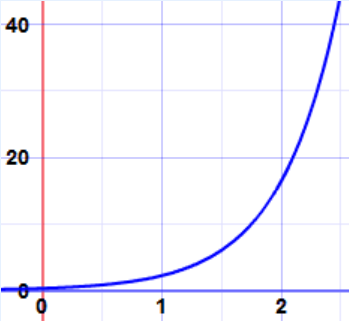
\includegraphics[width=0.3\textwidth]{images/expfigure.png}
  \caption{示例图片：用于演示 figure 环境与浮动管理}
  \label{fig:expfigure}
\end{figure}

图 \ref{fig:expfigure} 是当前目录下的 \texttt{expfigure.png}。
这里的 \texttt{[htbp]} 表示 LaTeX 可以将该图片放在“当前位置（here）、
页顶（top）、页底（bottom）或单独的浮动页（page）”。
因此，图片不一定严格出现在源码所在位置的正下方，
而是由 LaTeX 根据页面空间自动安排。

这种机制称为“浮动管理”。
它的优点是可以避免图片把正文挤得过于零碎，
从而使整篇文档的版面更整齐。
在较长的数学报告或课程论文中，
通常应当让 LaTeX 自动管理图表的位置，
而不是频繁手工调整。

\section{学习要求}

学生需要按时完成作业，
认真阅读教材，
并能够书写规范的定义、命题和证明。
本课程既重视计算训练，
也重视数学表述的严谨性。

\section{考核方式}

平时作业、课堂测验和期末考试共同构成总评成绩，
其中期末考试占主要比重。

\end{document}